\documentclass[tikz,border=5pt]{standalone}
\usepackage{amsmath}
\usetikzlibrary{arrows.meta, decorations.markings}

\begin{document}
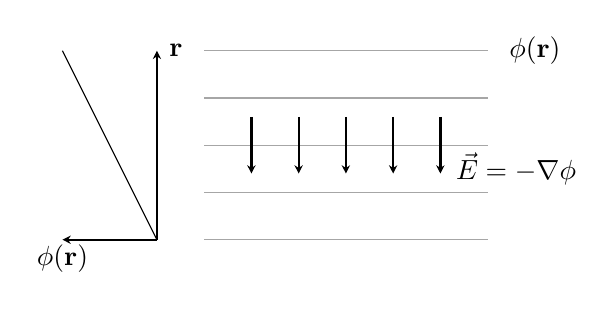
\begin{tikzpicture}[scale=1.2, >={Stealth[length=3pt,width=3pt]}]

% === E-veld uit scalaire potentiaal φ ===
% Equipotentiaalvlakken
\foreach \y in {1, 0.5, 0, -0.5, -1,}{
  \draw[gray!70] (-1.5,\y) -- (1.5,\y);
}

% E-veld vectoren
\foreach \x in {-1, -0.5, 0, 0.5,1}{
  \draw[->, thick] (\x,0.3) -- ++(0,-0.6);
}


%Grafiek phi
\draw[->,thick] (-2,-1)--(-2,1);
\draw[->,thick] (-2,-1)--(-3,-1);
\draw (-2,-1)--(-3,1);

% Labels
\node at (2,1) {$\phi(\mathbf{r})$};
\node at (1.8,-0.25) {$\vec{E} = -\nabla \phi$};
\node at (-3,-1.2) {$\phi(\mathbf{r})$};
\node at (-1.8,1) {$\mathbf{r}$};
\end{tikzpicture}
\end{document}